
\documentclass{beamer}
\usepackage{ifxetex}
\ifxetex
    \usepackage{fontspec}
    \usepackage{xunicode}
    \usepackage{xltxtra}
    \usepackage{xecyr}
    \usepackage{polyglossia}

    \setmainlanguage{english}
    \setotherlanguages{russian}
\else
    \usepackage[T1]{fontenc}
    \usepackage[utf8]{inputenc}
    \usepackage{lmodern}
\fi

%% USAGE: 
% \usepackage[logo=sklogo]{beamerskoltech} 
%   if you have a stand-alone image file for Sk logo 
% or
% \usepackage[logo]{beamerskoltech} 
%   if you has no logo-file, but want LaTeX to generate it. 
%   In this case you probably will need to use `--enable-write18 -interaction=nonstopmode` arguments running the latex command.
%   in papeeria and overleaf all works fine
% or 
% \usepackage{beamerskoltech}
%   In case you don't want logo at all 
%
% provided commands:
% color `skoltechgreen` -- the dark-green color for structure elements 
% command `\logoname` -- the name of logo file if exist 
% command `{\csk <text>}` -- the shortcut from `\color{skoltechgreen}`
% command `skfootnote{text}` -- put some text for current slide
% `\renewcommand{\skbeforetitle}{\vspace{-3ex}}` is useful in case you use `aspectratio=169`. Also for this aspectratio it is useful to make `\setlength{\skfootnotelen}{12cm}`
%%%%%%%%%%%%%%%%
\usepackage[logo=sklogo]{beamerskoltech} 
\usefonttheme[onlymath]{serif}

\usepackage{amsmath}
\usepackage{amssymb}
\usepackage{amsfonts}

\usepackage{hyperref}

\usepackage[natbib=true]{biblatex}
\usepackage{bibentry}
\usepackage{doi}
\addbibresource{references.bib}

\usepackage{tikz}
\usepackage{pgfplots}
\usetikzlibrary{calc}

\title{Geometric Deep Learning}
\subtitle{for Inverse Graphics}
\author{Serge Kozlukov}
\institute{Skoltech}
\date{June 5, 2020}

\begin{document}

\frame{\titlepage}

\begin{frame}\frametitle{Background}
    \begin{itemize}
            \item Hyperbolic DL
            \item Equivariant CNNs
            \item Graph-convolutional NNs
    \end{itemize}
\end{frame}

\begin{frame}{Background: Hyperbolic DL}
    \framesubtitle{Curvature bounds}

    \begin{itemize}
        \item \( M \) a metric space,
        \item \( p, q, r \in M \),
        \item \( \bar{p}, \bar{q}, \bar{r} \in \mathbb{R}^2 \) -- a comparison triangle,
        \item \( \gamma_t \in M \) on the geodesic between \( q, r \),
        \item \( |\bar{p}\bar{\gamma}_t| > |p\gamma_t| \):
    \end{itemize}

    \begin{figure}\centering
        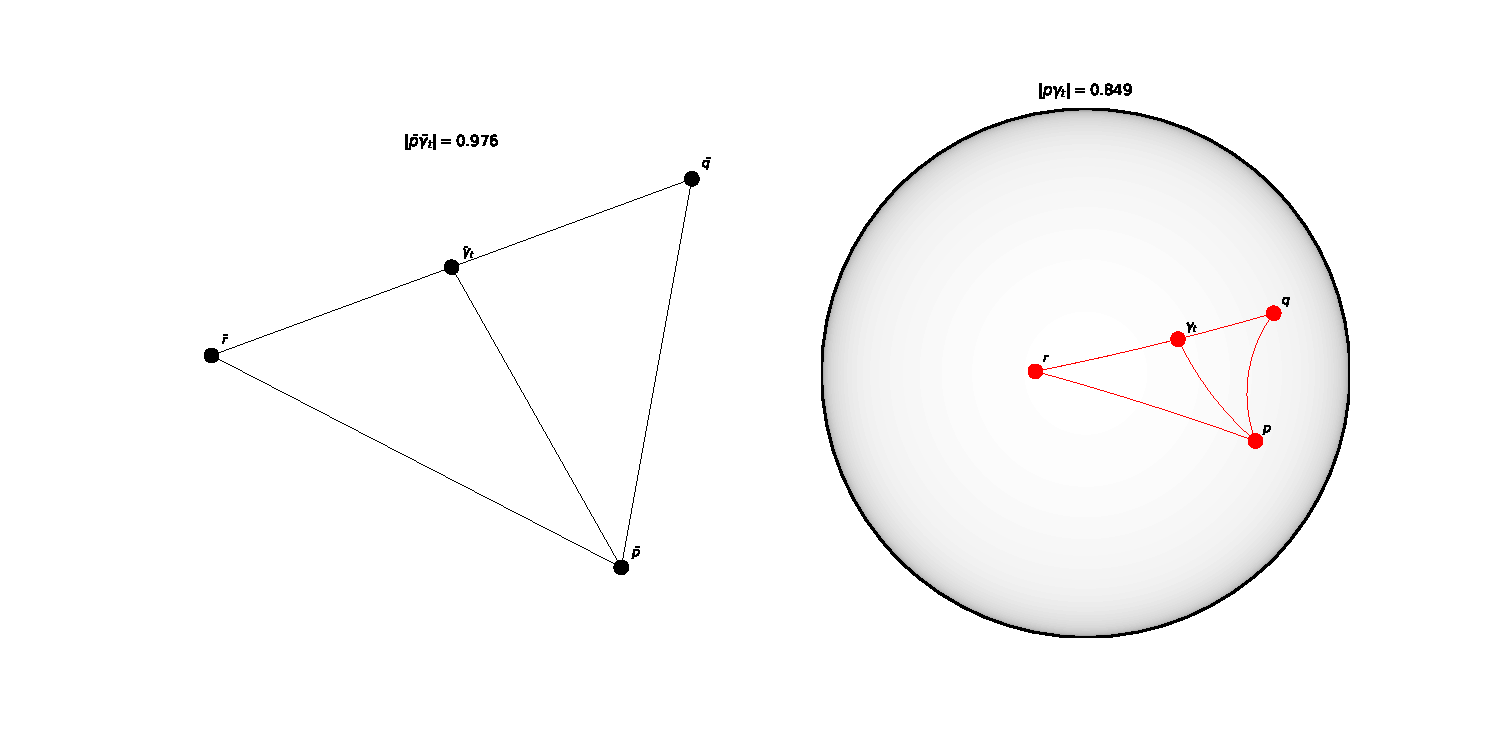
\includegraphics[width=.85\linewidth]{art/triangle-comparison.pdf}
    \end{figure}
\end{frame}

\begin{frame}{Background: Hyperbolic DL}
    \framesubtitle{Metric graphs}

    \begin{columns}
        \begin{column}{.45\linewidth}
            \begin{figure}\centering
                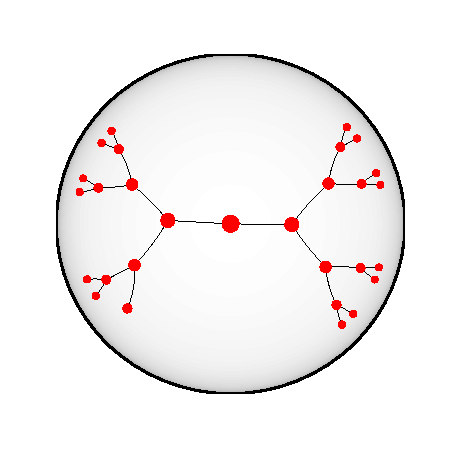
\includegraphics[width=.95\linewidth]{art/h-binary-tree.pdf}
                \caption{Binary tree: \( 2^{n+1}-1 \)
                points on first \( n \) levels}
            \end{figure}
        \end{column}
        \begin{column}{.45\linewidth}
            \begin{figure}\centering
                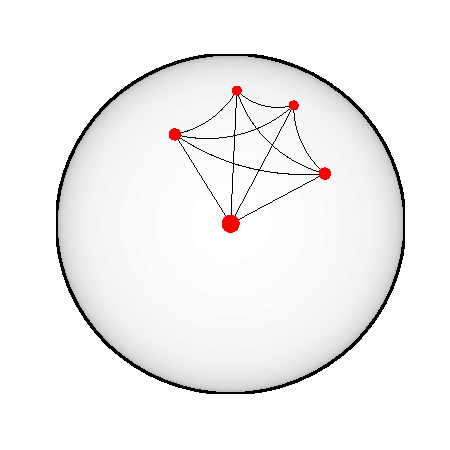
\includegraphics[width=.95\linewidth]{art/h-clique.pdf}
                \caption{Clique: \( n \) mutual nearest neighbours}
            \end{figure}
        \end{column}
    \end{columns}
\end{frame}

\begin{frame}{Background: Hyperbolic DL}
    \framesubtitle{Curvature in image classifiers}

    \begin{columns}
        \begin{column}{.5\linewidth}
            \begin{itemize}
                    \item ``Hyperbolic Image Embeddings''
                    \item Distance between embeddings is NPC
            \end{itemize}
        \end{column}
        \begin{column}{.5\linewidth}
            \begin{figure}\centering
                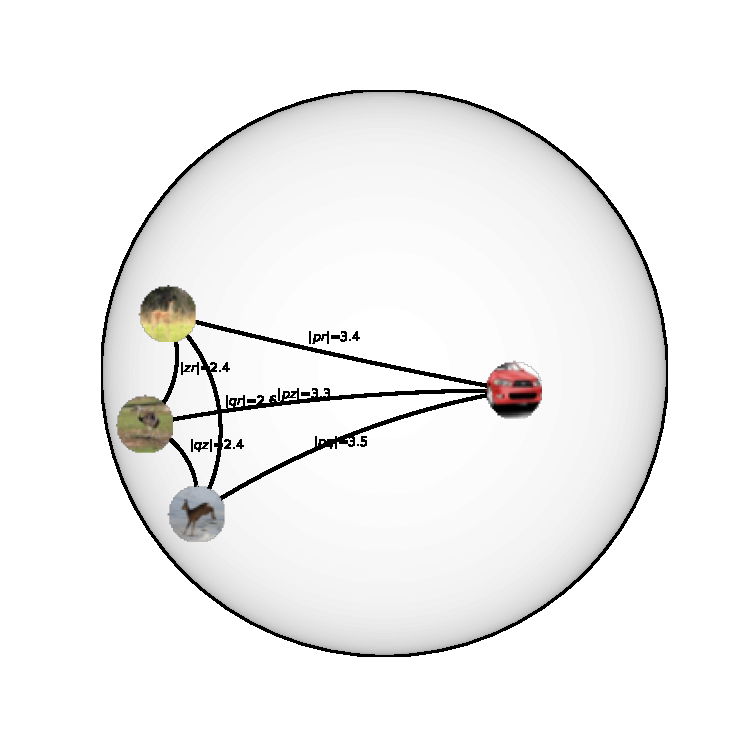
\includegraphics[width=.95\linewidth]{art/quadruple-8.pdf}
            \end{figure}
        \end{column}
    \end{columns}
\end{frame}

\begin{frame}{Background: Hyperbolic DL}
    \framesubtitle{Convolutions for ``hyperbolic arrays''}\centering

    \begin{figure}\centering
        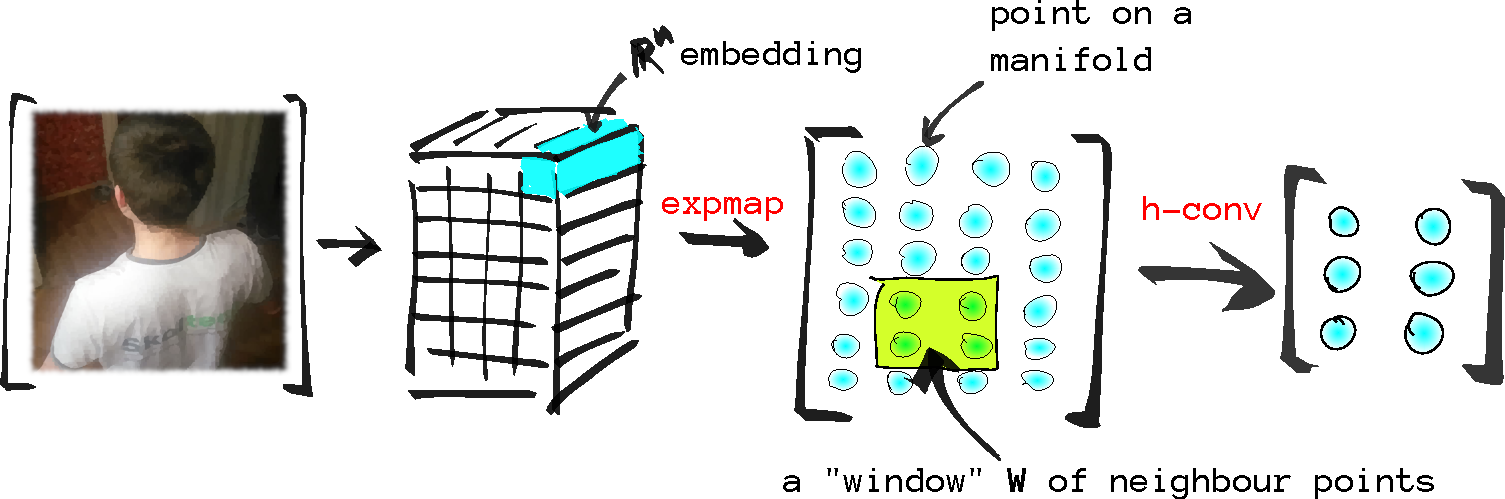
\includegraphics[width=\linewidth]{art/image-convolutions-2019.pdf}
    \end{figure}

        \[ x' = \exp_0\left(
            \operatorname{Conv2D}\left(
                \log_0(y)
                \right)\right) \]

        Kochurov, Karimov, Taktasheva, Mazur, Kozlukov
\end{frame}

\begin{frame}{Background}
    \framesubtitle{Equivariance}

    \[
        f \mathbin{*} g = x \mapsto \int_G f(g e) h(g^{-1} x) \operatorname{d}g
    \]

    \begin{itemize}
        \item Classic: \( (G, e, +, -), \) \( G=\mathbb{R}^n, \) \( e=0, \)
            \( g^{-1}x = x - g. \)
        \item \( * \) commutes with translations:
            \( g\circ (f \mathbin{*} h)
            = (g \circ f) \mathbin{*} h
            = f \mathbin{*} (g^{-1} \circ h). \)
        \item S2CNN (Cohen, Welling): \( \operatorname{dom}f = S^2, \)
            \( G = \operatorname{SO}(3) \).
    \end{itemize}
\end{frame}

\begin{frame}{Background: Deep Learning on Graphs}
    \framesubtitle{Message passing and EdgeConv}

    \begin{columns}
        \begin{column}{.45\linewidth}
            ``Message passing''
            \begin{itemize}
                    \item Edge list representation
                    \item \( x \) -- source
                    \item \( y \) -- destinations
                    \item \( m(x, y) \) -- ``message''
                    \item \( x' = \operatorname{Conv2D} m(x, y) \)
            \end{itemize}
            E.g. EdgeConv:
            \begin{itemize}
                \item \( m(x, y) = (x, y-x) \)
                \item PCDs: dynamic \( k \)-NN graph
            \end{itemize}
        \end{column}
        \begin{column}{.5\linewidth}
            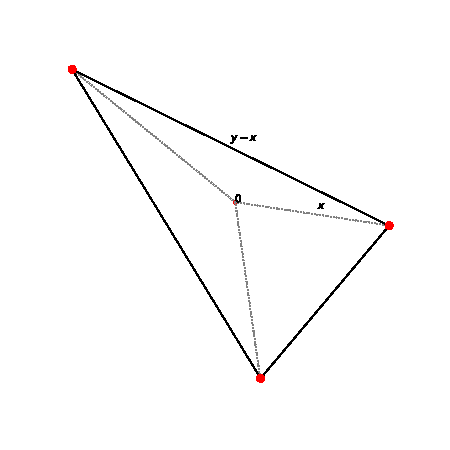
\includegraphics[width=\linewidth]{art/edgeconv-features.pdf}
        \end{column}
    \end{columns}
\end{frame}

\begin{frame}{Experiments and results}
    \framesubtitle{\texttt{H-Conv 0.2}: ``Relative Directions''}

    \begin{columns}
        \begin{column}{.45\linewidth}
            \texttt{H-Conv 0.1}:

            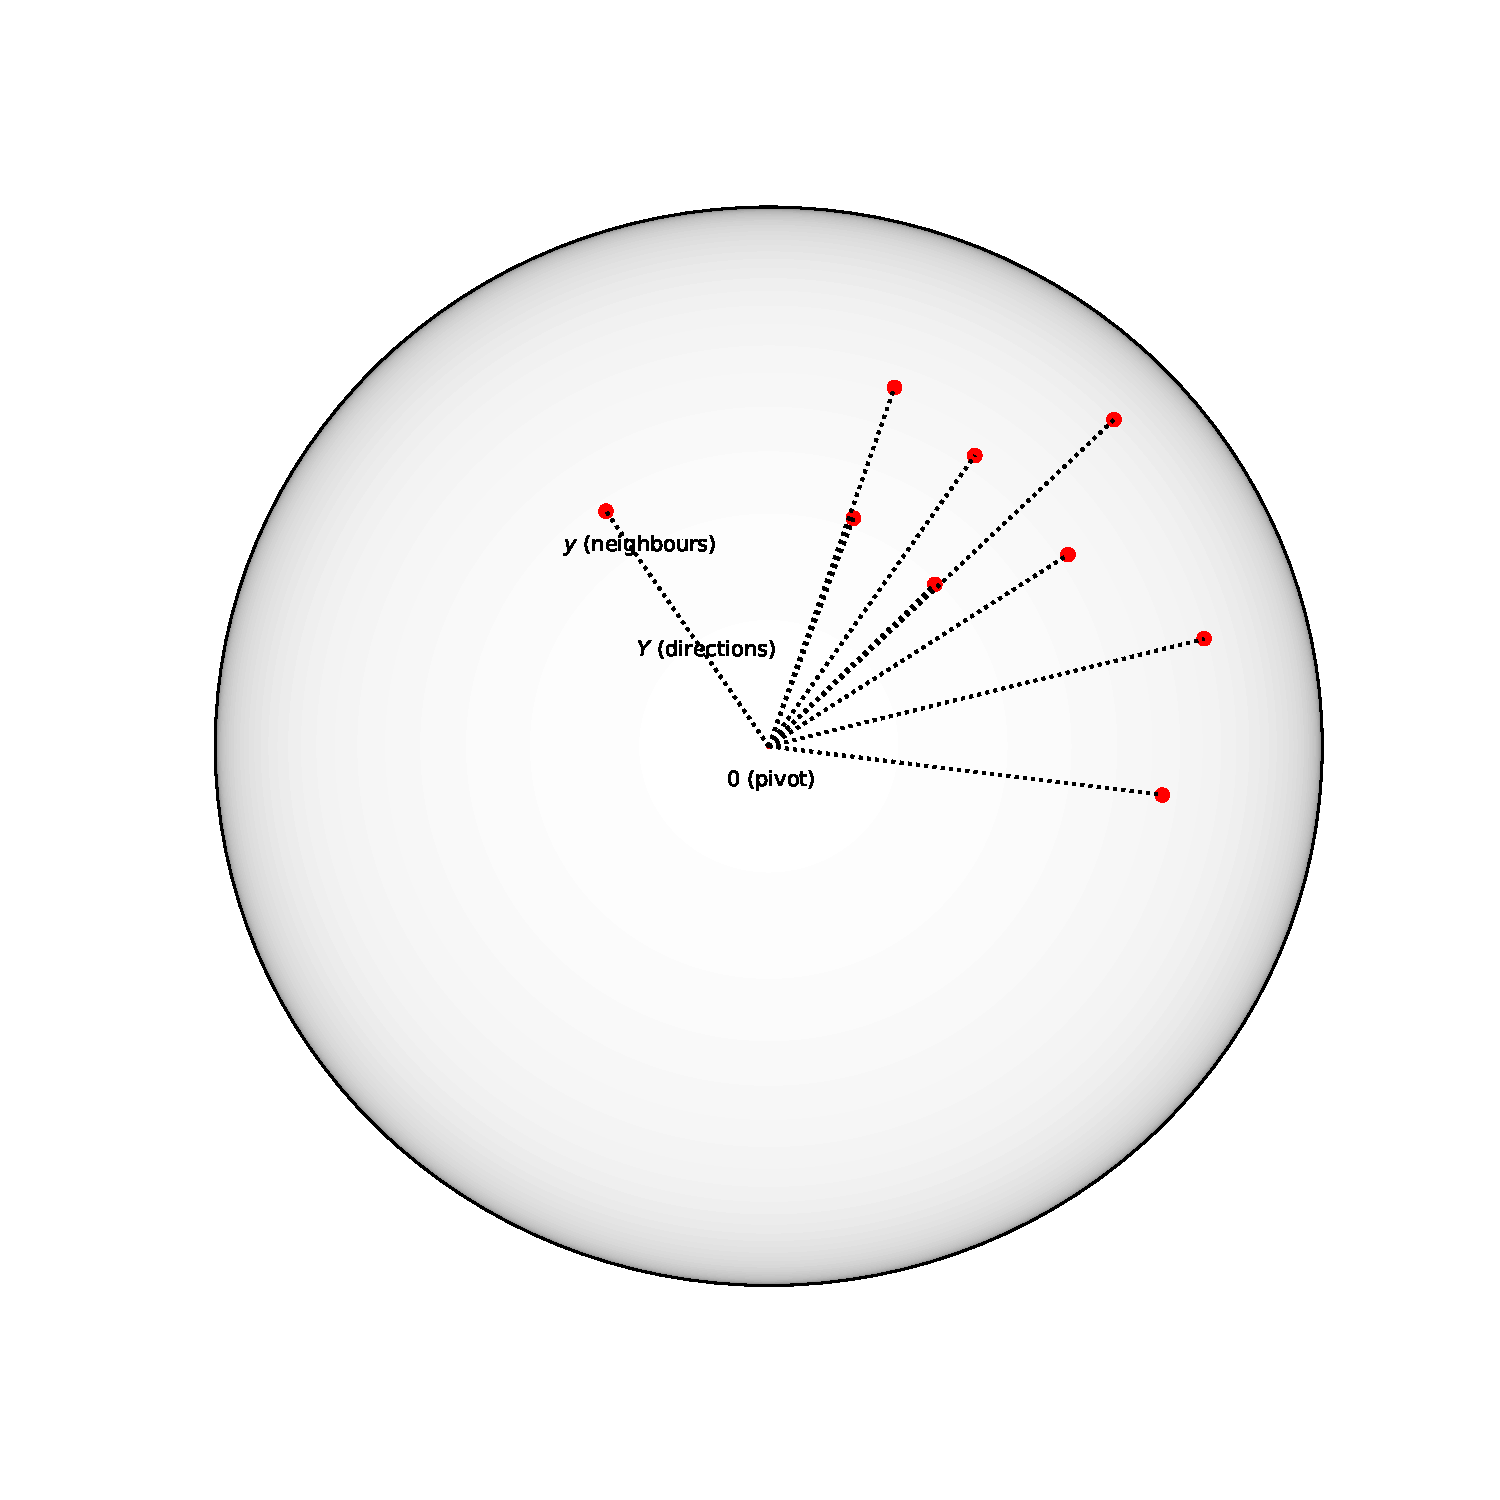
\includegraphics[width=.85\linewidth]{art/absolute-locations.pdf}
            \[ x' = \exp_0\left(
                \operatorname{Conv2D}\left(
                    \log_0 Y
                    \right)\right) \]
        \end{column}
        \begin{column}{.45\linewidth}
            \texttt{H-Conv 0.2}:

            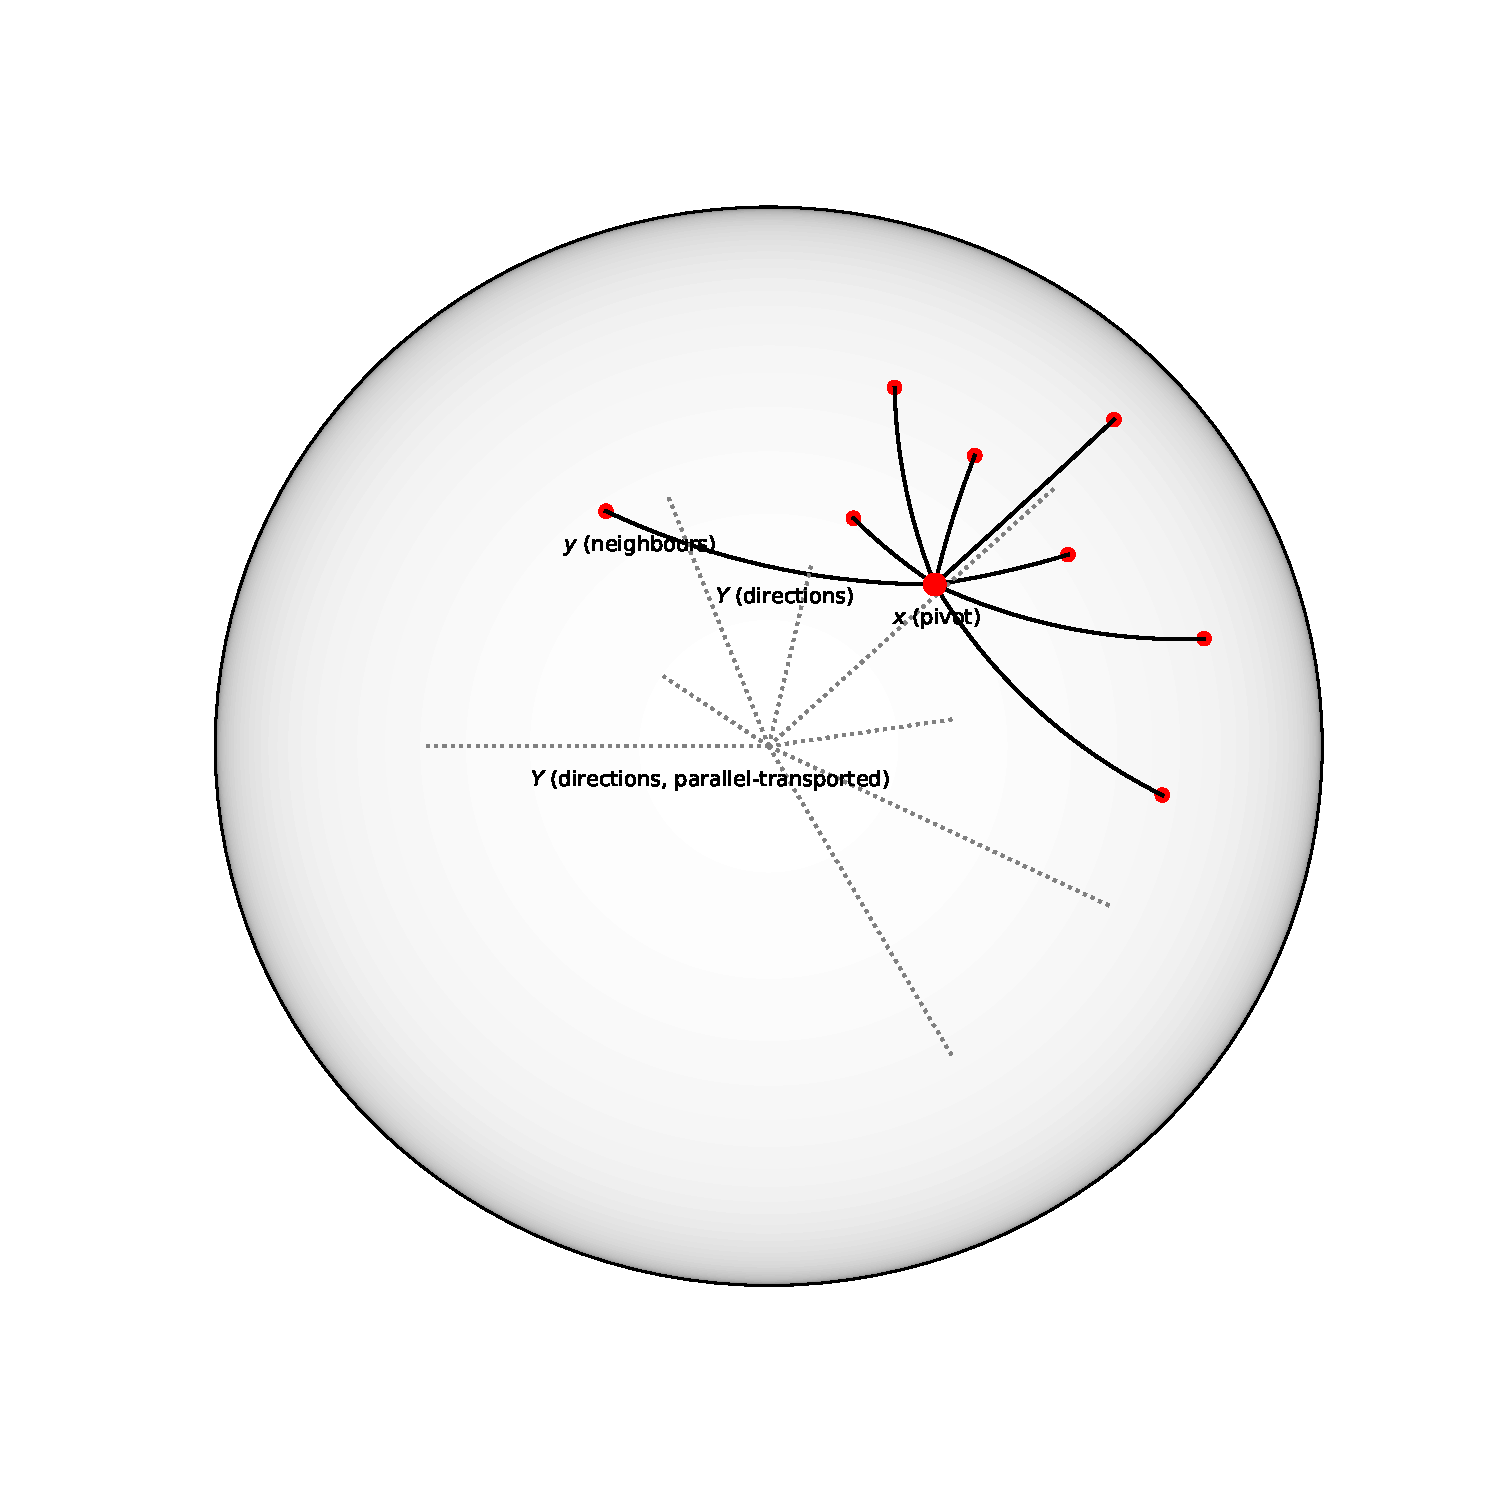
\includegraphics[width=.85\linewidth]{art/relative-locations.pdf}
            \[ x' = \exp_x\left(
                \operatorname{Conv2D}\left(
                    \log_x Y\right)\right) \]
        \end{column}
    \end{columns}
\end{frame}

\begin{frame}{Experiments and results}
    \framesubtitle{\texttt{H-EdgeConv}}

    \begin{columns}
        \begin{column}{.5\linewidth}\centering
                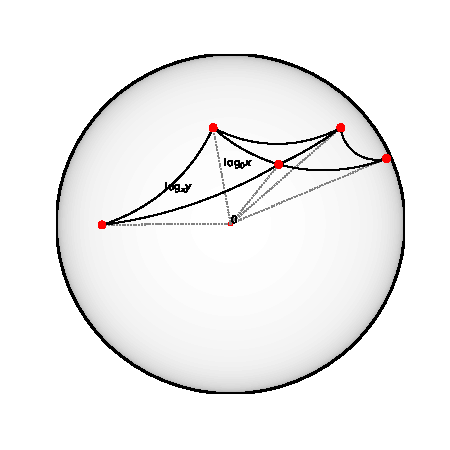
\includegraphics[width=.85\linewidth]{art/hedgeconv-features.pdf}
                \[\exp_o \operatorname{Conv2D}([\log_0x, \log_xy])\]
        \end{column}
        \begin{column}{.6\linewidth}
            \begin{table}[h!]
                \centering
                \begin{tabular}{|c c c c|} 
                    \hline
                    Model & params &
                    pts & acc
                    \\ [0.5ex] 
                    \hline\hline
                    \texttt{EdgeConv} & \( 1 \)M & \(1024\) & \(.90\)  \\ 
                    {\small 3DShapeNets} & \( 5 \)M & \(1024\) & \(.77\)  \\ 
                    \texttt{H-EdgeConv} & \( 85 \)K & 768 &  \( .71 \) \\ [1ex] 
                    \hline
                \end{tabular}
                \caption{Classification of Modelnet40 pointclouds}
            \end{table}

            \texttt{H-EdgeConv} is a combination of \texttt{H-Conv 0.\{1,2\}}
            plus \(k\)-NN graph instead of a regular grid of an image
        \end{column}
    \end{columns}
\end{frame}

\begin{frame}{Experiments and results}
    \framesubtitle{Publications}
    
    \begin{itemize}
        \item (ELLIS) geoopt,~\citet{geoopt}
        \item (under review) denoising,~\citet{denoisingAkhmedkhan}
    \end{itemize}
\end{frame}

\begin{frame}{Discussion}
    \begin{itemize}
        \item Points in the window (neighbourhood) -- ``a discrete signal on~\( \mathbb{D} \)'':
            \( \frac1n \sum_{i=1}^n \delta_{x_i} \)
        \item Other functional bases than \( \delta_x \)?~\cite{stollharmonic}
        \item \( \log_xy \) is only invariant wrt M\"obius addition
        \item \(x\mapsto \int_{\mathcal{A}} f(\phi~0) h(\phi^{-1}x) \operatorname{d}\phi \),
            more in~\cite{stollharmonic}
        \item Broader class of problems, e.g. correspondence detection\&description
    \end{itemize}
\end{frame}

\begin{frame}{Acknowledgements}
    Max Kochurov, Dmitry Ulyanov, Thibaut Le Gouic, Rasoul Karimov, and many,
    many others.
\end{frame}

\begin{frame}{References}
    \printbibliography
\end{frame}

\end{document}
